\begin{linenumbers*}
\label{app:emails}
\section{Communication with Danni}

\subsection{Valcon IT Strategy}
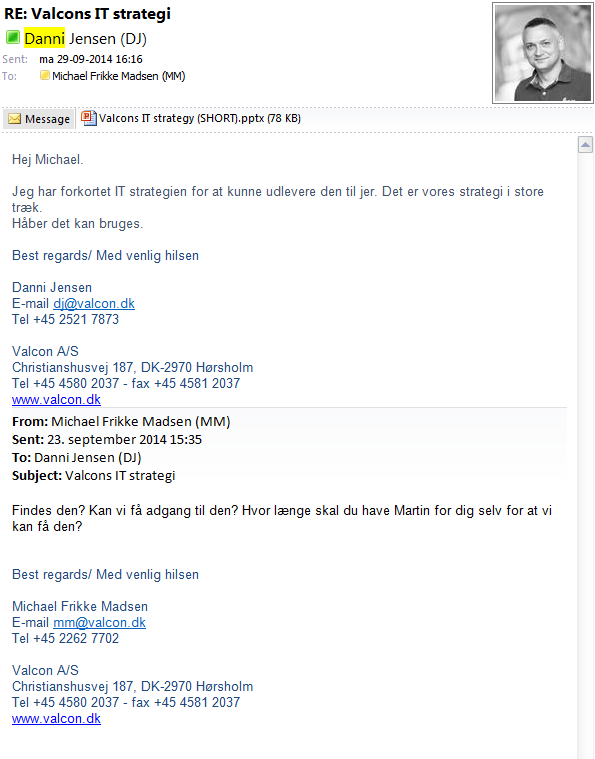
\includegraphics[width=1.36\textwidth]{appendix/danni_communication_1}

\subsection{Valcon Business Strategy}
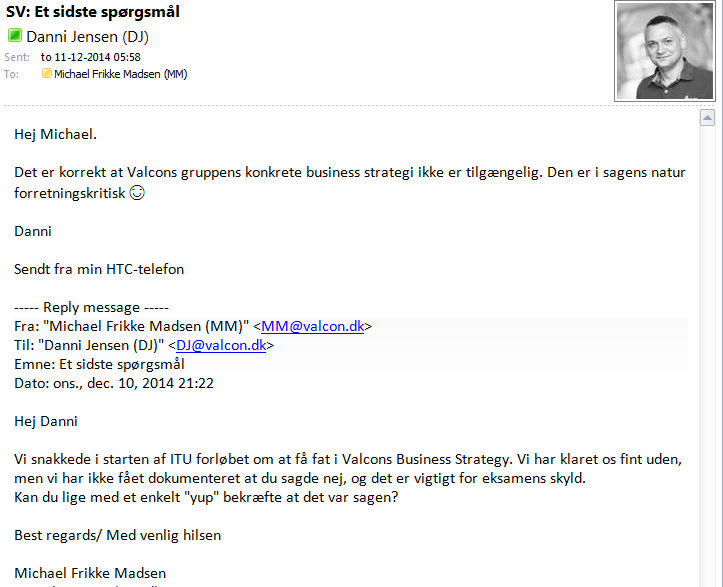
\includegraphics[width=1.36\textwidth]{appendix/danni_communication_2}

\subsection{Lync conversation 08-09-2014}
Michael Frikke Madsen (MM) [13:02]: 
Du må undskylde at jeg sådan presser på - vi skal bare helst have en bekræftelse på, om vi kan komme ud og holde et introducerende møde inden for de næste par uger, ellers skal vi til at kontakte andre virksomheder for at være sikre på at have noget, når vi reelt skal i gang :) \newline
Danni Jensen (DJ) [13:03]: 
Hej Michael. Det må I gerne, men I kommer selv til at stå for forløbet, forstået på den måde at I selv skal finde interessenter, spørge dem om tid osv
jeg skal selvfølgelig nok sparre med jer, men mit fokus er på Valcon og ikke projektet som sådan. Jeg skal nok komme med mine geniale input når I kommer med noget, men det er jer selv der skal være kreative og opsøgende

\subsection{Lync conversation 17-09-2014}
Michael Frikke Madsen (MM) [12:24]: 
Hey Danni. Vil du/Valcon foretrække dansk eller engelsk til vores rapport?
Vi kan begge dele, men er mest vant til engelsk til rapporter. \newline
Danni Jensen (DJ) [12:35]: 
Engrish pwease \newline
Michael Frikke Madsen (MM) [14:06]: 
Will do (y) \newline
Danni Jensen (DJ) [14:06]: 
Sweet

\subsection{Lync conversation 01-12-2014}
Michael Frikke Madsen (MM) [10:58]: 
Dav Danni
Vi sidder og skriver rapport, og vi skal for eksamens skyld bruge rygdækning til en enkelt ting:
Kan vi snakke/maile med en FO chef, som har erfaring i at ansætte?

Hvis svaret er nej, kan vi roligt skrive i rapporten at det ikke kunne lade sig gøre
Hvis svaret er ja, vil vi skrive en mail med nogle spørgsmål omkring hvad vedkomne ved om ansættelsesprocessen. \newline
Danni Jensen (DJ) [12:47]: 
Hej Michael. Jeg tror det bliver svært at klemme tid ud af en FO chef, de er ikke så gode til at give tid til noget der ikke giver dem opgaver \newline
\linelabel{line:danni_says_no_to_recruiter_interview}
Michael Frikke Madsen (MM) [12:55]: 
Det er i orden - det var også det vi havde gået ud fra, men vi opdagede at vi egentlig ikke havde nogen dokumentation på hvorfor vi ikke havde gjort det 

\section{Communication with Peter}

\subsection{Time Estimation}
\label{app:peter_time_estimation}
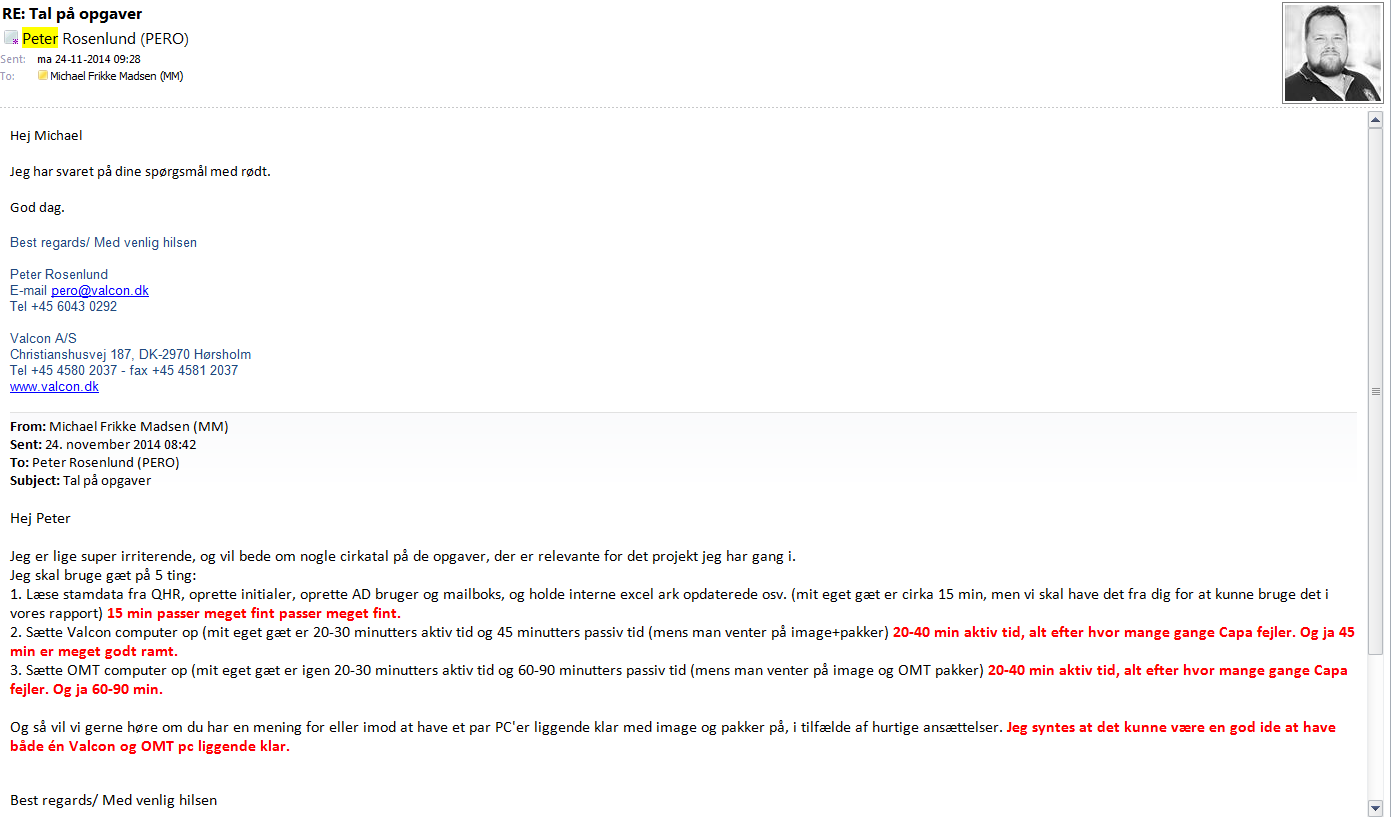
\includegraphics[width=1.36\textwidth]{appendix/peter_communication_1}

\section{Communication with Lisbeth}

\subsection{Time Estimation}
\label{app:lisbeth_time_estimation}
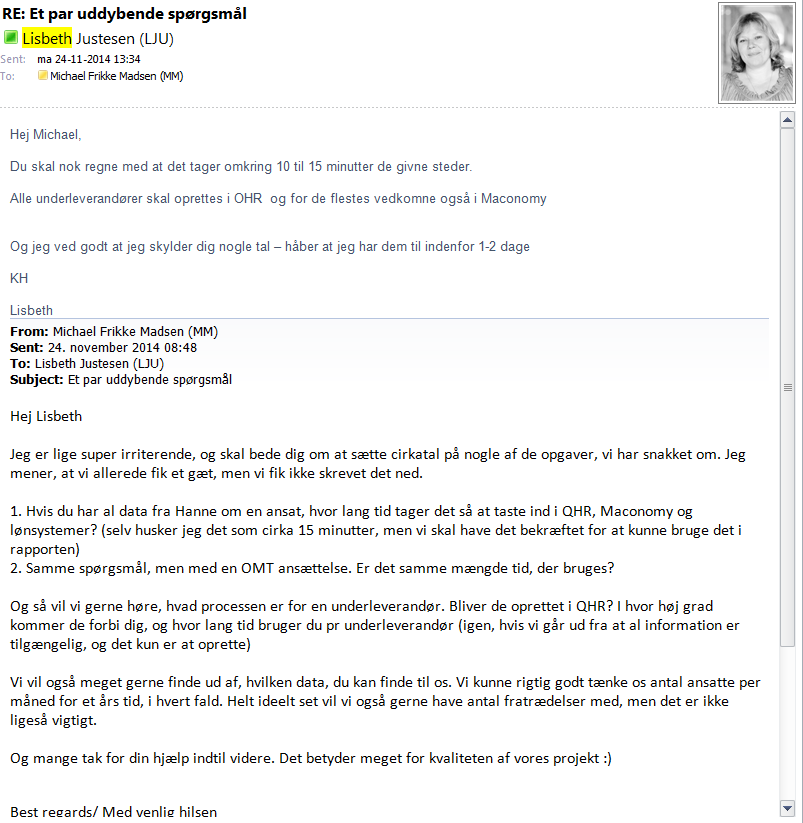
\includegraphics[width=1.36\textwidth]{appendix/lisbeth_communication_1}

\subsection{Data on Hires and Resignations}
\label{app:hires_and_resignations}
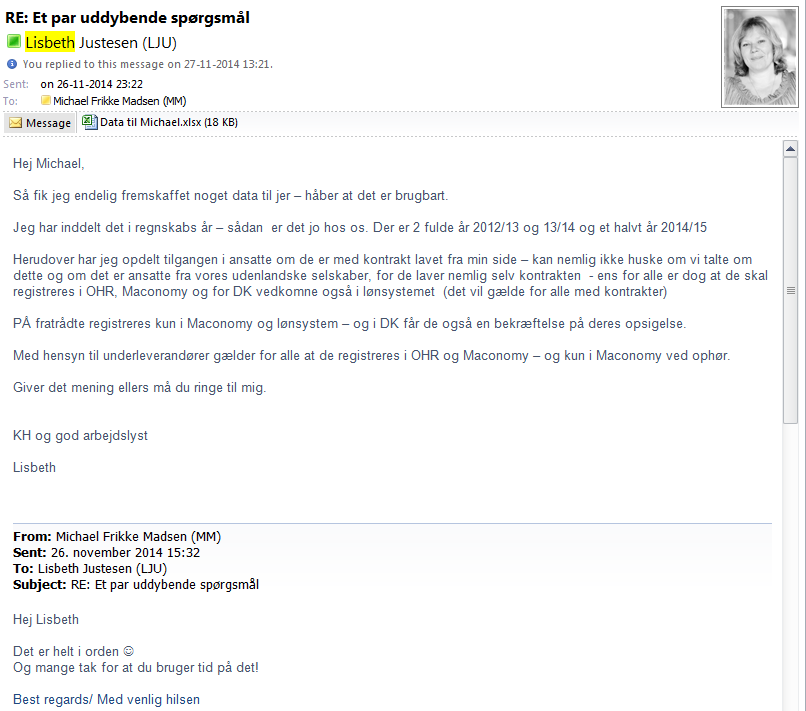
\includegraphics[width=1.36\textwidth]{appendix/lisbeth_communication_2}


\section{Communication with Hanne}

\subsection{Time Estimation}
\label{app:hanne_time_estimation}
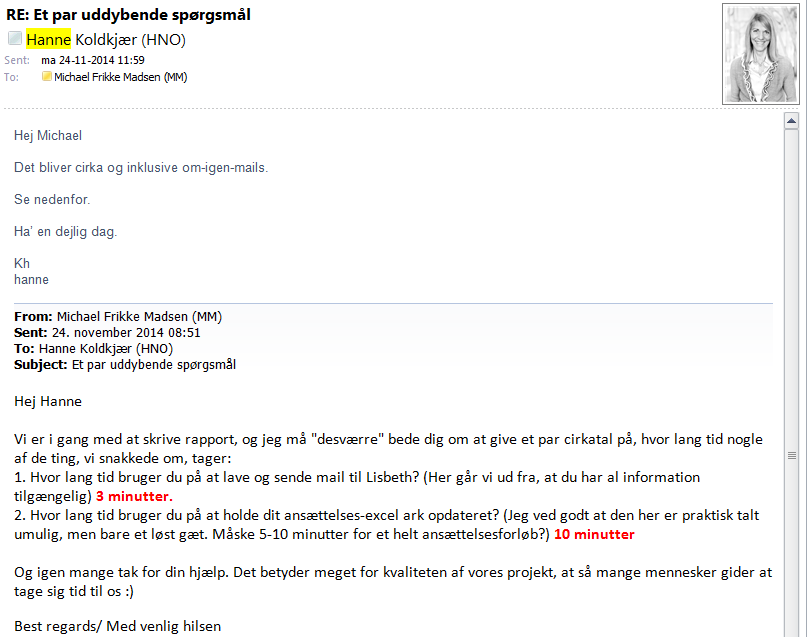
\includegraphics[width=1.36\textwidth]{appendix/hanne_communication_1}


\section{Communication with Jytte}

\subsection{Time Estimation}
\label{app:jytte_time_estimation}
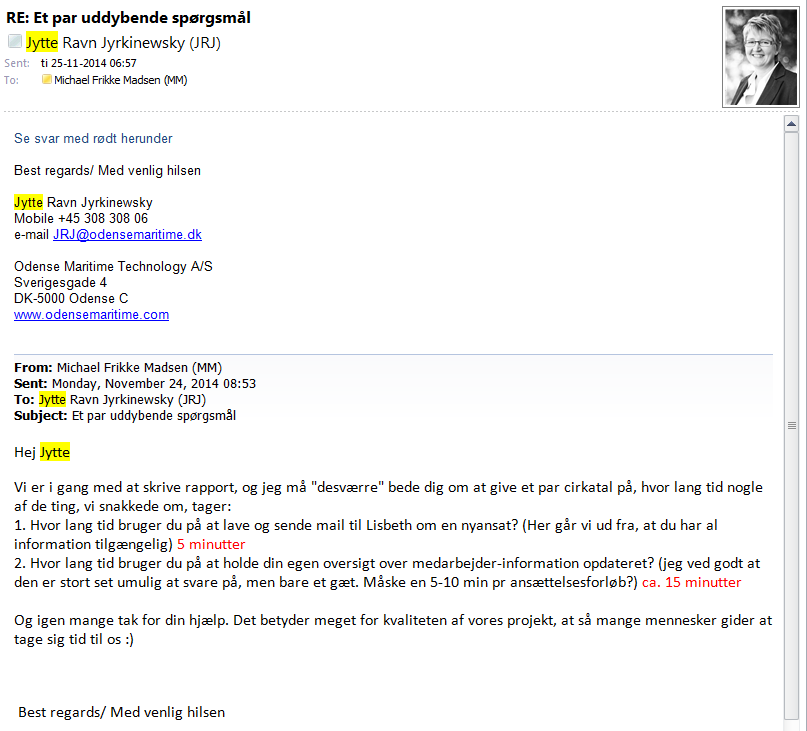
\includegraphics[width=1.36\textwidth]{appendix/jytte_communication_1}

\section{Communication with others}

\subsection{Question to another student help about structure in IT}
\linelabel{matias_on_structure}
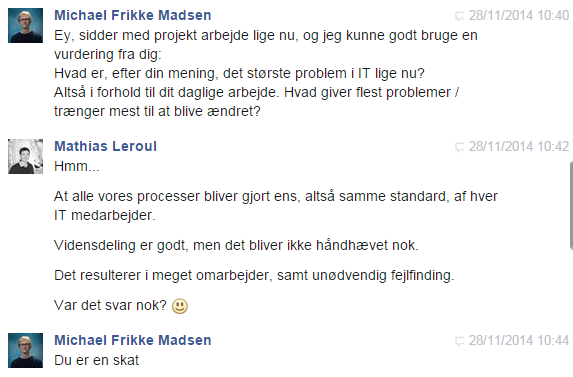
\includegraphics[width=1.36\textwidth]{appendix/other_communication_1}
\end{linenumbers*}
